\documentclass{article}
\usepackage{graphicx}
\usepackage[utf8]{inputenc}
\usepackage{amsmath}
\usepackage{enumitem}
\setlist[description]{style=nextline}

\begin{document}
\setlength\parindent{0pt}

\begin{titlepage}
\begin{center}

% Upper part of the page. The '~' is needed because \\
% only works if a paragraph has started.

\textsc{\LARGE Technische Universität Dresden}\\[1.5cm]

\textsc{\Large WS2014}\\[0.5cm]

% Title
{ \huge \bfseries Networks, Function and Genomics\\[0.4cm] }

% Author and lecturer
\noindent
\begin{minipage}{0.4\textwidth}
\begin{flushleft} \large
\emph{Author:}\\
Jan\\
Marc\\
Sebastian\\
\end{flushleft}
\end{minipage}%
\begin{minipage}{0.4\textwidth}
\begin{flushright} \large
\emph{Lecturer:} \\
Prof. Michael \textsc{Schroeder}
\end{flushright}
\end{minipage}

\vfill

% Bottom of the page
{\large \today}

\end{center}
\end{titlepage}

Als Programm wird benutzt
Cytascape

\section{Vorlesung}

\subsection{Graphen}
Grundlagen der Graphentheorie wurde von Euler mittels Königsberger Brücker gelegt.
\\
\fbox{
\begin{tabular}{l l}
Def:&Graph\\
&Ein Graph ist\\ 
&G= (V, E) \\
&V: Vertex (Knoten)\\
&E: Edges (Kanten)\\
\end{tabular}
}
\\ 

Graphen werden unter anderem für Kürzeste Wege, Zustandbasierten Spielen (z.B. Schach), Ausführreihenfolgen, Abhängigkeiten, Zustandsautomaten, Stammbaum, Genregulierung usw. eingesetzt.
\\

\fbox{
\begin{tabular}{l l}
Def:&Skalenfrei (Scalefree)\\
&Rich get Richer \\
\end{tabular}
}
\\

\fbox{
\begin{tabular}{l l}
Def:& Degree Distribution\\
&Wie verteilt sich die Anzahl der Nachbarn auf die Anzahl der Knoten. Meist sieht dies so aus.\\ 
\end{tabular}
}
\\

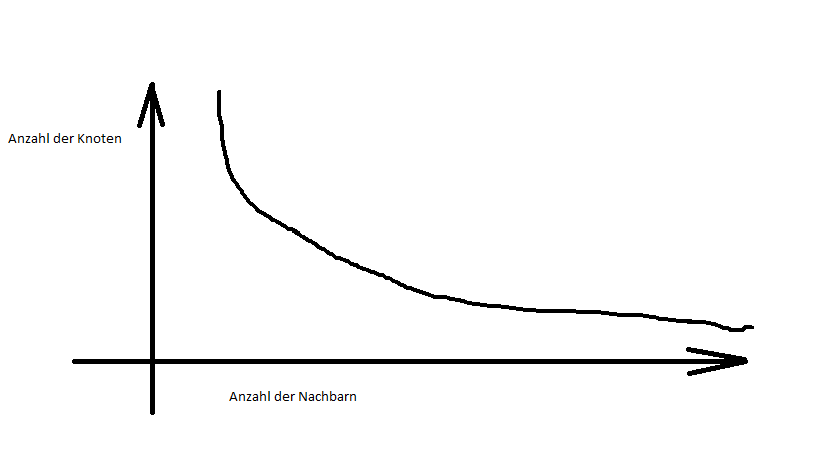
\includegraphics[scale=0.5]{scalefree}\\
\fbox{
\begin{tabular}{l l}
Def:&Performel Preferenz (? Name vll nicht richtig)\\
&Die mehr haben, kriegen mehr. The rich get richer\\
\end{tabular}
}

\subsection{Proteinnetze}
Artikel: Wie ein Biologe ein Radio untersuchen würde\\

Die Daten gibt es seit 15 Jahren. PDB (Protein database) Enthält 3D Protein Strukturen.\\

Wie weit geht die Wechselwirkung zwischen den Proteinen?\\

Es gibt verschiedene Analyseverfahren:\\


Veraltete (ca 2000):
\begin{enumerate}
  \item Über die Distanz
  \item Wie viel Oberfläche wird durch die Interaktion überdeckt
\end{enumerate}

Problem der Analyse der Überdeckung: Es gibt wenige 3D Strukturen. \\


Aktuelle PPI Methoden (ab ca 2003): 
\begin{enumerate}
  \item PPB
  \item Y2H (Yeast 2 Hybrid)
  \item AP/MS (Afinity prificention with mass spectrometry)
\end{enumerate}

\subsubsection{Y2H}
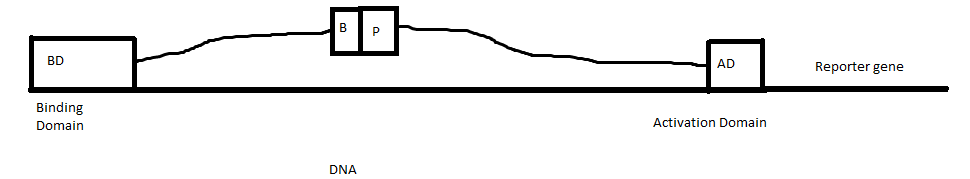
\includegraphics[scale=0.5]{Y2H}\\

Erst wenn irgentwas passiert, passiert irgentwas. In Hefekulturen -> Sequenzierung.

Vorteil:
Interaktion die nicht stark sind, können detektiert werden. 

Nachteil:
Komplexe Interaktion mit mehreren Proteinen sind schwierig zu detektieren.
Findet immer in Hefe statt

\subsubsection{AP/MS (Afinity prificention with mass spectrometry)}
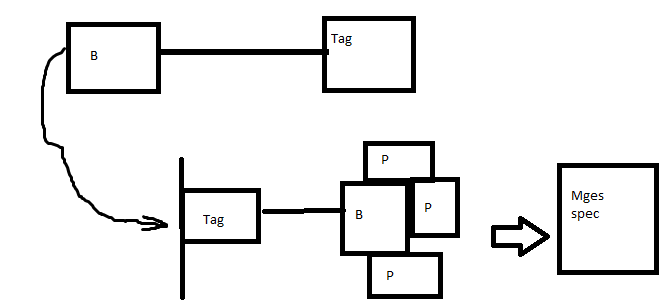
\includegraphics[scale=0.5]{APMS}\\
\begin{tabular}{r l}
P:&Proteinen\\
B:&Der Köter an dem die Proteine binden\\
Tag:&Wird an eine Oberfläche gebunden\\
\end{tabular}
\\

Schätzungen zufolge gibt es 600.000 Interaktion im Menschlichen Körper\\

Zusammenfassung\\
Netzwerk spielen überall eine wichtige Rolle\\

Wichtige Datenbanken\\
String (EMBL): Enthält alles (Über Gene), ist die Wichtigste\\
HPRD: Daten werden Manuell gepflegt\\
Biogrid\\
Intact\\
DIP\\
\\

Damit sind viele Daten verfügbar. Darauf kann man die Algorithmen loslassen.\\
\\

Fragen zu Graph\\
Wo ist das Zentrum\\
Wer ist der wichtigste Knoten (laut Degree Distribution)\\
Wo gut sind lokale Gruppen verdrahtet\\
\\

\fbox{
Def Clique:
Teil das Graphen, in dem Jeder knoten mit jedem anderen verbunden ist. 
}
\\

\fbox{
Def Clusterindex\\
}
\\

Ci = $\frac{2n}{ki * (ki – 1)}$\\
ki: Anzahl der Nachbarn\\
n: Zahl der Kanten zwischen den Nachbarn\\
\\

Cluterindex = 1  $\leftrightarrow$ Clique\\
\\

Je mehr Nachbarn desto schwieriger ist es einen hohen Cluster index zu erhalten\\
\\

Offen (Was noch nachgetragen werden muss)\\
Hub\\
Barizentrum (? Name vll falsch)\\


\newpage
\section{Vorlesung}
Paper: Google goes Cancer


Page Rank. Kommt aus Italien wurde von google genutzt. In Page Rank kommt gibt es einen Score. Dieser Score ist umso höher je mehr Seiten auf die Ziel Seite Verlinken. 
Gibt Ausschluss über die Qualität der Daten. Bestimmte Gene können ausgefiltert werden. Suche nach Master regulatoren (Gene die viele Gene beeinflussen). 

Kürzeste Pfade um Wirkstoffe zu finden. Gene  verändern ihre Aktivität durch Medikamente. Dies tun sie aber nicht sofort. Finde den Wirkstoff, der die  kürzesten Pfade hat.

Von Knoten i nach j zu gehen. 

mij = 1 / |N(vi)|
N(vi): Nachbarn von Knoten vi


Stationärer Zustand
M * x = Lambda * x
M: Stationärer Zustand 
x: Konfiguration
Lambda: Ein Scalarer Wert

Power Methode

$M^n * x0 $\\
Das ganze konvergiert. 

Zusätzlich gibt es noch einen zufälligen Neustart. 


Erstellung eines Zufälligen Graphen

Eingabe:
Anzahl Vertexes
Anzahl Edges

Algorithmus:
Erstelle die Vertexes.
Verbinde zufällig 2 Vertexes zu einer Edge. Solang bis es genug edges gibt

Erder Schring Modell (? Name evt. Nicht richtig)
Das Modell wie die Degree Distribution in einem Zufälligen Graph aussieht. Die ist eine Gaus Verteilung. 


Erstellen eines Scale Free netzwerkes
Eingabe:
Anzahl Vertexes
Anzahl Edgeverteilung.

Algorithmus (? Habe nicht aufgepasst)


In Netzwerken kann man Motive finden. Diese kann man für die Kompression nutzen. Ein paar Beispiele sind unten angegeben.\\
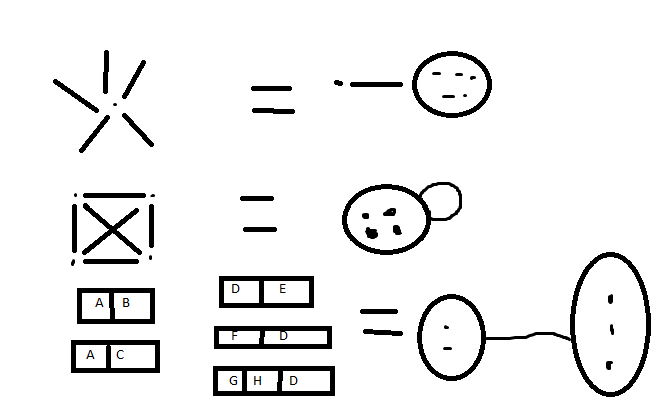
\includegraphics[scale=0.5]{graphvereinfachungen}\\

Offene Fragen:
Hethrow Situation

\newpage
\section{Vorlesung - PowerGraphs}
Graphen zur Analyse von Biologischen Prozessen. 

Für diese Vorlesung wird es auf der Website drei Papers und die Präsentation geben.
\subsection{from network quality to drug repositioning}
Bis 2000 war der Forschungsschwerpunkt die Untersuchung von einem spezifischen Gen.
Die Komplexen Zusammenhänge wurden kaum bis gar nicht betrachtet. 
2001 Änderte sich dies mit einer Veröffentlichung von Jeong in der "Nature"\footnote{siehe Präsentation Seite 2}. 
Der Informationsgewinn hatte hier aber seine Grenzen, da dieser Graph schwer analysierbar war.
\\

"Comprehension is compression" - Gregory Chainitin 
\\

Wie kann Kompression bei einem Komplexen Graphen erreicht werden?\footnote{siehe Präsentation Seite 5}
\begin{description}
  \item[Hubs in networks]\hfill\\ Da es sich meist um Skalenfrei Graphen handelt könnte man Greedy vorgehen.
  \item[Protein Complexes]\hfill\\ Cliquen können ebenfalls komprimiert werden.
  \item[Domain and morif-based interactions]\hfill\\ Bi-Cliquen werden auch vereinfacht.
\end{description}

Diese neue Struktur hat aber auch Nachteile. Es können neue Informationen gewonnen werden, es gehen vielleicht auch
Informationen verloren.
\\

Wie erstellt man so einen Graphen?\footnote{Siehe Präsentation Seite 7; Diese Heuristik kann noch optimiert werden.}\\
Eventuell Greedy über Anzahl der Knoten oder Pfadlänge? $\rightarrow$ Problem: Potenzmenge muss betrachtet werden.\\
\begin{enumerate}
  \item Verbesserung hierzu: Da bei der Erstellung von Powerknoten nur direkte Nachbarn in Frage kommen müssen
        auch nur diese bei der Erstellung betrachtet werden. $\rightarrow$ Nun haben wir eine quadratische Komplexität.\\
  \item Nach der ersten Kategorisierung werden die Potenzkanten nach ihrer Mächtigkeit sortiert.\footnote{Siehe Seite 7 B}
  \item Bei der weiteren Vernetzung müssen entweder alle Knoten im Potenzknoten enthalten sein. Falls dies nicht der
        Fall wäre müsste man die Punkte raus nehmen die nicht überlappen. \footnote{Siehe Seite 7 D}\\
        Die neuen Vernetzungen müssen in die Liste aufgenommen werden.
  \item Bei der Zusammenfassung können Redundanzen entstehen.\footnote{Siehe Seite 7 E} Falls dies auftritt können die
        entsprechenden Knoten aus den Potenzknoten herausgenommen werden.
  \item Falls Fall D und E nicht auftreten, haben wir den Power Graphen.
\end{enumerate}
Bei der Analyse der Power Graphen konnte festgestellt werden, dass Potenzknoten oft zur selben Domäne gehören
(Bei Cliquen) oder die Funktion bei stark vernetzten Knoten ähnlich sind oder sie eine gemeinsame Funktion haben.
\footnote{Siehe Seite 8} 

\subsection{Network compression as quality measure}
Die Kompression kann als Qualitätsmerkmal des Graphen herangezogen werden.
\footnote{Siehe Seite}\\
Problem hierbei ist, dass diese Kompression  größenabhängig ist, keine
Information über Kompressionsart enthält oder die Einordnung der Kompressionsrate
ist. \\
Das Problem der Kategorisierung der Ergebnisse ist, dass beim Test oft die
Ergebnisse nicht Binär sind (zum Beispiel: interagiert oder interagiert nicht).
Das Rauschen bei den Test könnte kein zufälliges Rauschen sein. (Jan: Ich bin
mir nicht sicher, ob ich das richtig verstanden habe.)
\footnote{Siehe Seite "Uniform Noise Model" ff}\\
Eine Kategorisierung kann auch anhand von Publizierten, gut erforschten Netzwerken
festlegen. Dieses lässt sich an itoCore und itoFull erkennen.\\

\subsection{Exkurs 1. Vorlesung}
\subsubsection{AP/MS screening}
\fbox{%
  \begin{minipage}{1\textwidth}
    \begin{description}
      \item[AP/MS] \hfill \\ Tag bindet an Protein B. Tag wird an Glasplatte befestigt. Proteine
      bindet an Protein B.\\
    \end{description}
  \end{minipage}
}
Lässt sich meist gut komprimieren. His tag + cDNA führt manchmal zu schlechten
Ergebnissen.
\subsubsection{Y2H}
Lässt sich schlecht komprimieren.\footnote{Siehe Präsentation}
\subsubsection{Scalable two-phase pooling strategy}
Besser als Y2H. Schlechter als AP/MS.\footnote{Siehe Präsentation}
\subsection{Complete and accurate networks}
In Biologie kaum komplette und richtige Netzwerke vorhanden. Das Kompressionsverfahren
Lässt sich aber auch auf alle anderen Graphen anwenden. Beispiele für die Kompression
lässt sich auch in der Präsentation finden.
\subsection{Completing incomplete bi-cliques}
Nur echte Bi-Cliquen werden komprimiert, was kann man tun falls fast eine komplette
Clique vorhanden ist? $\rightarrow$ Verlinkung hinzufügen. Das Problem ist hier,
dass dies nicht Verlustfrei ist. Also muss man abwiegen wie wahrscheinlich diese
Clique ist. \footnote{Vergleiche Algorithmus aus der Präsentation}
\subsubsection{Drug-Target-Disease Network}
Medikamente werden mit Zielproteine und Krankheiten in Verbindung gebracht.
Wenn man bei diesen Graphen die Bi-Cliquen vervollständigt steigt die 
Kompressionsrate.\footnote{Siehe Seite 43} Dies hat auch im biologischen
Vorteile. Ein anderes Beispiel ist die Vervollständigung des Graphen mit den
Herzerkrankungen und dem Parasiten Medikamenten.\\
Wenn man die Struktur der Medikamente oder die Bindestruktur vergleicht, lassen
sich Gemeinsamkeiten erkennen. $\rightarrow$ Das spricht für die Vervollständigung.

\newpage
\section{Vorlesung - Anwendung von Pagerank}
In dieser Vorlesung wird die Frage behandelt inwieweit man den Pagerank auf die biomedizinische Themen anwenden und diesen vergleichen kann.

\subsection{Einleitung}
In der heutigen Zeit ist es ein Ziel Vorhersagen und Unterscheidung von Krankheitsverläufen feststellen zu können und dementsprechend Medizin für die Unterschiede bereit zustellen (Individualisierte Medizin). Doch wie kann man den spezifischen Krankheitsverlauf beeinflussen und behandeln? Das Problem an dieser Verfahrensweise sind die klinischen Test, welche ein Medikament erst durchlaufen muss. Bei der Individualisierten Medizin braucht man, wie sonst auch, Versuchsgruppen die groß genug sind um eine signifikante Aussage zu geben.\\
Z.B. die Unterscheidung bei der Überlebensrate von Krebs (über ein Kapler-Meyer-Plot\footnote{Siehe Seite 5}). So fand man sieben Gene welche zu einer 70\% Wahrscheinlichkeit vorhersagen wie der Krebs verlaufen wird. Unter anderen gibt es in diesen Genen eins, welches einen sehr großen Teil der anderen Gene beeinflusst und reguliert.\\
Ein weiterer Forschungsgegenstand ist der, dass man aus allen möglichen biologischen Publikationen Relationen aus allen Entitäten erstellt. Damit möchte man herausfinden in welcher Art und Weise und ob Proteine überhaupt mit einander interagieren und sich beeinflussen.\\
Aus den Zusammenhängen aus den Nebeneffekten von Medikamenten können Profile für diese Medikamente erstellt werden. Diese zeigen, auf was ein Medikament alles reagiert. Daraus können ebenfalls Ontologien aufgebaut werden.
\subsection{Anwendung des Pagerank in biomedizinischen Anwendungen(Netrank)}
Wenn nun also der Netrank auf Proteinnetzwerke angewendet werden soll stellen sich folgende Fragen:
\begin{itemize}
\item[-] Wie definiert man einen guten oder schlechten Krankheitsverlauf?
\item[-] Wie bestimmt man die Bewertung für solche?
\item[-] Wie vergleicht man diese Bewertungen miteinander und unter welchen Maßstab?
\end{itemize}
\subsubsection{Vorhersagen durch Genexpressionen}
Bisher wird zur Krebsuntersuchung ein Eingriff gemacht, bei dem Krebszellen aus dem Körper entnommen werden müssen. Das Ziel ist, dass diese Vorhersagen nicht durch einen Eingriff sondern durch die einfache Blutabnahme oder Speichelprobe getätigt werden kann.\footnote{Siehe Seite 10} Bei Blut ist dann aber die Frage, wie etwas, was ich untersuchen möchte überhaupt im Blut zirkuliert. Wie hoch muss die Konzentration sein um eine Aussage treffen zu können?\\
Bei der Analyse der Gene bei Patienten besteht ein Problem darin, dass man meist nicht viele Testfälle hat. Dementsprechend kann es dadurch zu einem Overfitting des angelerntes Algorithmus kommen.
\subsubsection{Finden von relevanten Gene in einem Netzwerk}
Wie verhindert man, dass beim Pagerank ein Knoten eine Senke ist. Dementsprechend könnte man nie aus diesem Knoten herauskommen. Für diesen Fall wurde der Damping factor eingeführt, welcher sagt, dass man zu einer gewissen Wahrscheinlichkeit an einem zufällig ausgewählten Knoten neu anfängt.\\
Netrank hat die Hauptidee, dass man das Netzwerk mittelt und dadurch Spitzen heraus nimmt.\footnote{Siehe Seite 20} Dieser ist auch im Vergleich zu klassischen Methoden besser.\footnote{Siehe Seiten 24, 31}
%\begin{itemize}
%\item[Fold Change] Es werden zufällige Gene ausgewählt und diese zum Entscheide genommen. Aber diese werden nicht                                                               untereinander verglichen. Dies kann dazu führen, dass man Gene mit genau der selben Verhaltensweise aussucht, doch diese bringen keinen Vorteil für die Entscheidung.
%\end{itemize}
%\subsection{Validierung von Daten}
\subsection{Qualität der Vorhersage}
Man könnte annehmen, dass, je höher die Signatur ist, desto besser ist die Genauigkeit, doch dies ist nicht der Fall. Desweiteren kann man auch mit der Testpatitienten Anzahl vergleichen.\footnote{Siehe Seite 29}\\
Verbessert nun Netrank wirklich das Ergebnis? Dies hängt von mehreren Faktoren ab. Unter anderem auch an dem Damping Factor.
\subsubsection{Damping factor}
Es wurde getestet welcher Damping Factor die besten Vorhersagen treffe.\footnote{Siehe Seite 33} Man kann erkennen das es zwei verschiedene Gruppen gibt. Eine, die bei einem kleinen Damping Factor gut vorherbestimmen und die anderen, die dies bei einem hohen tun. Da stellt sich nun aber die Frage ob die Netzwerke mit einem kleineren Damping Factor besser werden, wenn diese Netzwerke verbessert und vervollständigt werden.
\subsection{Wie einzigartig sind Signaturen}
Wir vergleichen zwei Hypothesen: Jeder Krebs ist anders und somit sollten Signaturen sich nicht überschneiden. gegen Krebsarten haben gewisse Gemeinsamkeiten, damit sollten die Signaturen zu einem gewissen Grad überschneiden.\footnote{Siehe Seite 38}
\subsection{Zussammenfassung}
Netzwerke können helfen Krankheiten vorrauszusagen. Dafür braucht man Gen Expressionsdaten. Mit den richtigen Algorithmen und ... 


\end{document}
